\documentclass[11pt]{article}
\usepackage{geometry}
\usepackage[utf8]{inputenc}
\usepackage[english]{babel}
\usepackage{amsmath}
\usepackage{amssymb}
\usepackage{amsfonts}
\usepackage[
    pdftex, 
    dvipsnames
]{xcolor}
\usepackage[
    colorlinks=true,
    linkcolor=black,
    urlcolor=Thistle
]{hyperref}
\usepackage{fancyhdr}
\usepackage{datetime}
\usepackage{xargs}
\usepackage{ccicons}
\usepackage{mdframed}
\usepackage{caption}
\usepackage{cancel}
\usepackage[nottoc]{tocbibind}
\usepackage[
    outputdir=.texpadtmp
]{minted}
\usepackage[parfill]{parskip}

% ==== License =====
\usepackage[
    type={CC}, 
    modifier={by-nc-sa}, 
    version={4.0},
]{doclicense}

% ==== todo notes ====
\usepackage[
    colorinlistoftodos,
    prependcaption,
    textsize=tiny
]{todonotes}
\newcommandx{\note}[2][1=]{\todo[linecolor=Thistle,backgroundcolor=Thistle!25,bordercolor=Thistle,#1]{#2}}
\newcommandx{\unsure}[2][1=]{\todo[linecolor=red,backgroundcolor=red!25,bordercolor=red,#1]{#2}}
\newcommandx{\change}[2][1=]{\todo[linecolor=blue,backgroundcolor=blue!25,bordercolor=blue,#1]{#2}}
\newcommandx{\info}[2][1=]{\todo[linecolor=OliveGreen,backgroundcolor=OliveGreen!25,bordercolor=OliveGreen,#1]{#2}}

% General
\newcommand{\mc}[1]{\mathcal{#1}}

% Math Bold Font, Vector Notations
\newcommand{\ba}{\mathbf{a}}
\newcommand{\bb}{\mathbf{b}}
\newcommand{\bc}{\mathbf{c}}
\newcommand{\bd}{\mathbf{d}}
\newcommand{\be}{\mathbf{e}}
\renewcommand{\bf}{\mathbf{f}}
\newcommand{\bg}{\mathbf{g}}
\newcommand{\bh}{\mathbf{h}}
\newcommand{\bi}{\mathbf{i}}
\newcommand{\bj}{\mathbf{j}}
\newcommand{\bk}{\mathbf{k}}
\newcommand{\bl}{\mathbf{l}}
\newcommand{\bm}{\mathbf{m}}
\newcommand{\bn}{\mathbf{n}}
\newcommand{\bo}{\mathbf{o}}
\newcommand{\bp}{\mathbf{p}}
\newcommand{\bq}{\mathbf{q}}
\newcommand{\br}{\mathbf{r}}
\newcommand{\bs}{\mathbf{s}}
\newcommand{\bt}{\mathbf{t}}
\newcommand{\bu}{\mathbf{u}}
\newcommand{\bv}{\mathbf{v}}
\newcommand{\bw}{\mathbf{w}}
\newcommand{\bx}{\mathbf{x}}
\newcommand{\by}{\mathbf{y}}
\newcommand{\bz}{\mathbf{z}}
\newcommand{\bzero}{\mathbf{0}}

% Proofs, Structures
\newcommand{\proof}{\tit{\underline{Proof:}}} % This equivalent to the \begin{proof}\end{proof} block
\newcommand{\proofforward}{\tit{\underline{Proof($\implies$):}}}
\newcommand{\proofback}{\tit{\underline{Proof($\impliedby$):}}}
\newcommand{\proofsuperset}{\tit{\underline{Proof($\supseteq$):}}}
\newcommand{\proofsubset}{\tit{\underline{Proof($\subseteq$):}}}
\newcommand{\contradiction}{$\longrightarrow\!\longleftarrow$}
\newcommand{\qed}{\hfill $\blacksquare$}

% Number Spaces, Vector Space
\newcommand{\R}{\mathbb{R}}
\newcommand{\real}{\mathbb{R}}
\newcommand{\complex}{\mathbb{C}}
\newcommand{\field}{\mathbb{F}}

% customized commands
\newcommand{\settag}[1]{\renewcommand{\theenumi}{#1}}
\newcommand{\tbf}[1]{\textbf{#1}}
\newcommand{\tit}[1]{\textit{#1}}
\newcommand{\overbar}[1]{\mkern 1.5mu\overline{\mkern-1.5mu#1\mkern-1.5mu}\mkern 1.5mu}
\newcommand{\double}[1]{\mathbb{#1}} % Set to behave like that on word
\newcommand{\trans}[3]{$#1:#2\rightarrow{}#3$}
\newcommand{\map}[3]{\text{$\left[#1\right]_{#2}^{#3}$}}
\newcommand{\dime}[1]{\mathrm{dim}(#1)}
\newcommand{\mat}[2]{M_{#1 \times #2}(\R)}
\newcommand{\aug}{\fboxsep=-\fboxrule\!\!\!\fbox{\strut}\!\!\!}
\newcommand{\basecase}{\textsc{\underline{Basis Case:}} }
\newcommand{\inductive}{\textsc{\underline{Inductive Step:}} }
\newcommand{\norm}[1]{\left\lVert#1\right\rVert}
\newcommand{\independent}{\perp \!\!\! \perp}

% Set section number in front of equation enumerations
\counterwithin{equation}{section}
\counterwithin{footnote}{section}
\author{\ccLogo\,\, Tingfeng Xia}
\title{\textsc{CSC317/418 Computer Graphics}}
\date{Winter Term, 2021}

\begin{document}
\maketitle
\doclicenseThis
\section*{Information}
\begin{itemize}
	\item Starting winter term 2021, Computer Graphics will be switching from its previous course code CSC418 to CSC317. 
	\item Course webpage: \url{https://github.com/karansher/computer-graphics-csc317}
	\item This note contains figures from Prof. Karan Singh's lecture slides. It also might contain figures by Marschner and Shirley and David Levin. 
	\item Textbook: Shirley, P., \& Marschner, S. (2009). \textit{Fundamentals of Computer Graphics (Third Edition)}. 
\end{itemize}
\tableofcontents


%%%%%%%%%%%%%%%%%%%%%
% Raster Images
%%%%%%%%%%%%%%%%%%%%%
\section{Raster Image}
An image is a distribution of light energy on a 2D film. Digital images today are represented as rectangular arrays of pixels. 
\subsection{Raster Devices}
\subsubsection{Raster Displays} These are displays that are comprised of a certain number of pixel units. Each of these pixel units contains three subpixels - red, green, and blue. When we say a display is $1920 \times 1080$, we mean that the display has that many pixels in the two directions, this also means that we have, at subpixel level, $1920 \times 1080 \times 3$ ``elements'' on the display. 

\subsubsection{Raster Input Devices}
The raster input filter we will introduce is Bayer Filter. In each pixel of a Bayer Filter, there is only one color - either red, green, or blue. Due to the nature of human eyesight, we are more sensitive to the color green. Hence, the Bayer Filter has twice green elements as compared to red and blue.\footnote{Patterns to the Bayer Filter may vary. The one presented in slides is BGGR.}

\subsubsection{Data Types for Raster Images}
Storage for $1024^2$ image (1 megapixel)
\begin{itemize}
	\item bitmap: 128KB, 
	\item grayscale 8bpp: $1024^2 \times 8 / 8 / 1024^2 = $1MB, 
	\item grayscale 16bpp: $1024^2 \times 16 / 8 / 1024^2 = $2MB, 
	\item color 24bpp: 3MB, \footnote{24bpp means 24 bits per pixel, so 8 bits for each color: 0 - 255}
	\item floating point high dynamic range color: 12MB
\end{itemize}

\subsubsection{Gamma Correction}
On a display, the intensity is non-linear with respect to input intensity. The Gamma correction relationship is formularized as 
\begin{equation}
	\text{display intensity} = \text{max display intensity} a^\gamma
\end{equation}
where $a$ is the amplitude from the image in the range in $[0, 1]$. The $\gamma$ is what we can set, usually in display settings. To set the right gamma correction, we need to find image amplitude that is equal to half of the display's brightness, then
\begin{equation}
	\frac{1}{2} = a^\gamma \quad 
	\implies \quad
	\gamma = \frac{\ln .5}{\ln a}
\end{equation}

\subsubsection{Modelling Transparency}
Simple RGB is great, but that only gets us solid colours, meaning that we cannot model transparency information with it. RGBA addresses this by simply appending an alpha channel variable to the end of the original triplet, making it a RGBA quadruple. We will also need this for the Porter/Duff Composition described below. 

\subsection{Image Composition}
Compositing is about layering images on top of one another. But there are many ways to do the composition, i.e. which image goes at the top and how you handle places with transparency. The Porter/Duff Composition\footnote{\url{http://ssp.impulsetrain.com/porterduff.html}} is a unified approach for this problem. 

Suppose we have two images source and destination. We we try to combine these two images, each pixel of the result can be divided into four regions: Both, Source, Dest, and Neither. The formula for this operation is a linear combination of contents of the four regions, where the weights are the ares of each region: 
\begin{equation}
	A_{src}[s] + A_{dest}[d] + A_{both}[b] 
\end{equation}
where
\begin{itemize}
	\item $[s]$ is either 0 or the color of the source pixel, 
	\item $[d]$ is either 0 or the color of the destination pixel, 
	\item $[b]$ is either 0, the color of the source pixel or the color of the destination pixel.
\end{itemize}
With the alpha channel being interpreted as coverage, the areas are given by these formulas: 
\begin{align}
	&A_{src} = \alpha_s (1 - \alpha_d) \\
	&A_{dst} = \alpha_d (1 - \alpha_s) \\
	&A_{both} = \alpha_s \alpha_d
\end{align}
The alpha channel of the result is computed in a similar way: 
\begin{equation}
	A_{src} [as] + A_{dest} [ad] + A_{both} [ab]
\end{equation}
where 
\begin{itemize}
	\item $[as]$ and $[ad]$ are either 0 or 1 depending on whether the source and destination regions are present, and 
	\item $[ab]$ is 0 when both regions is blank (transparent), and 1 otherwise. 
\end{itemize}
The Porter/Duff operations table in Figure \ref{porter duff} shows all 12 possible scenarios. 
\begin{figure}
	\center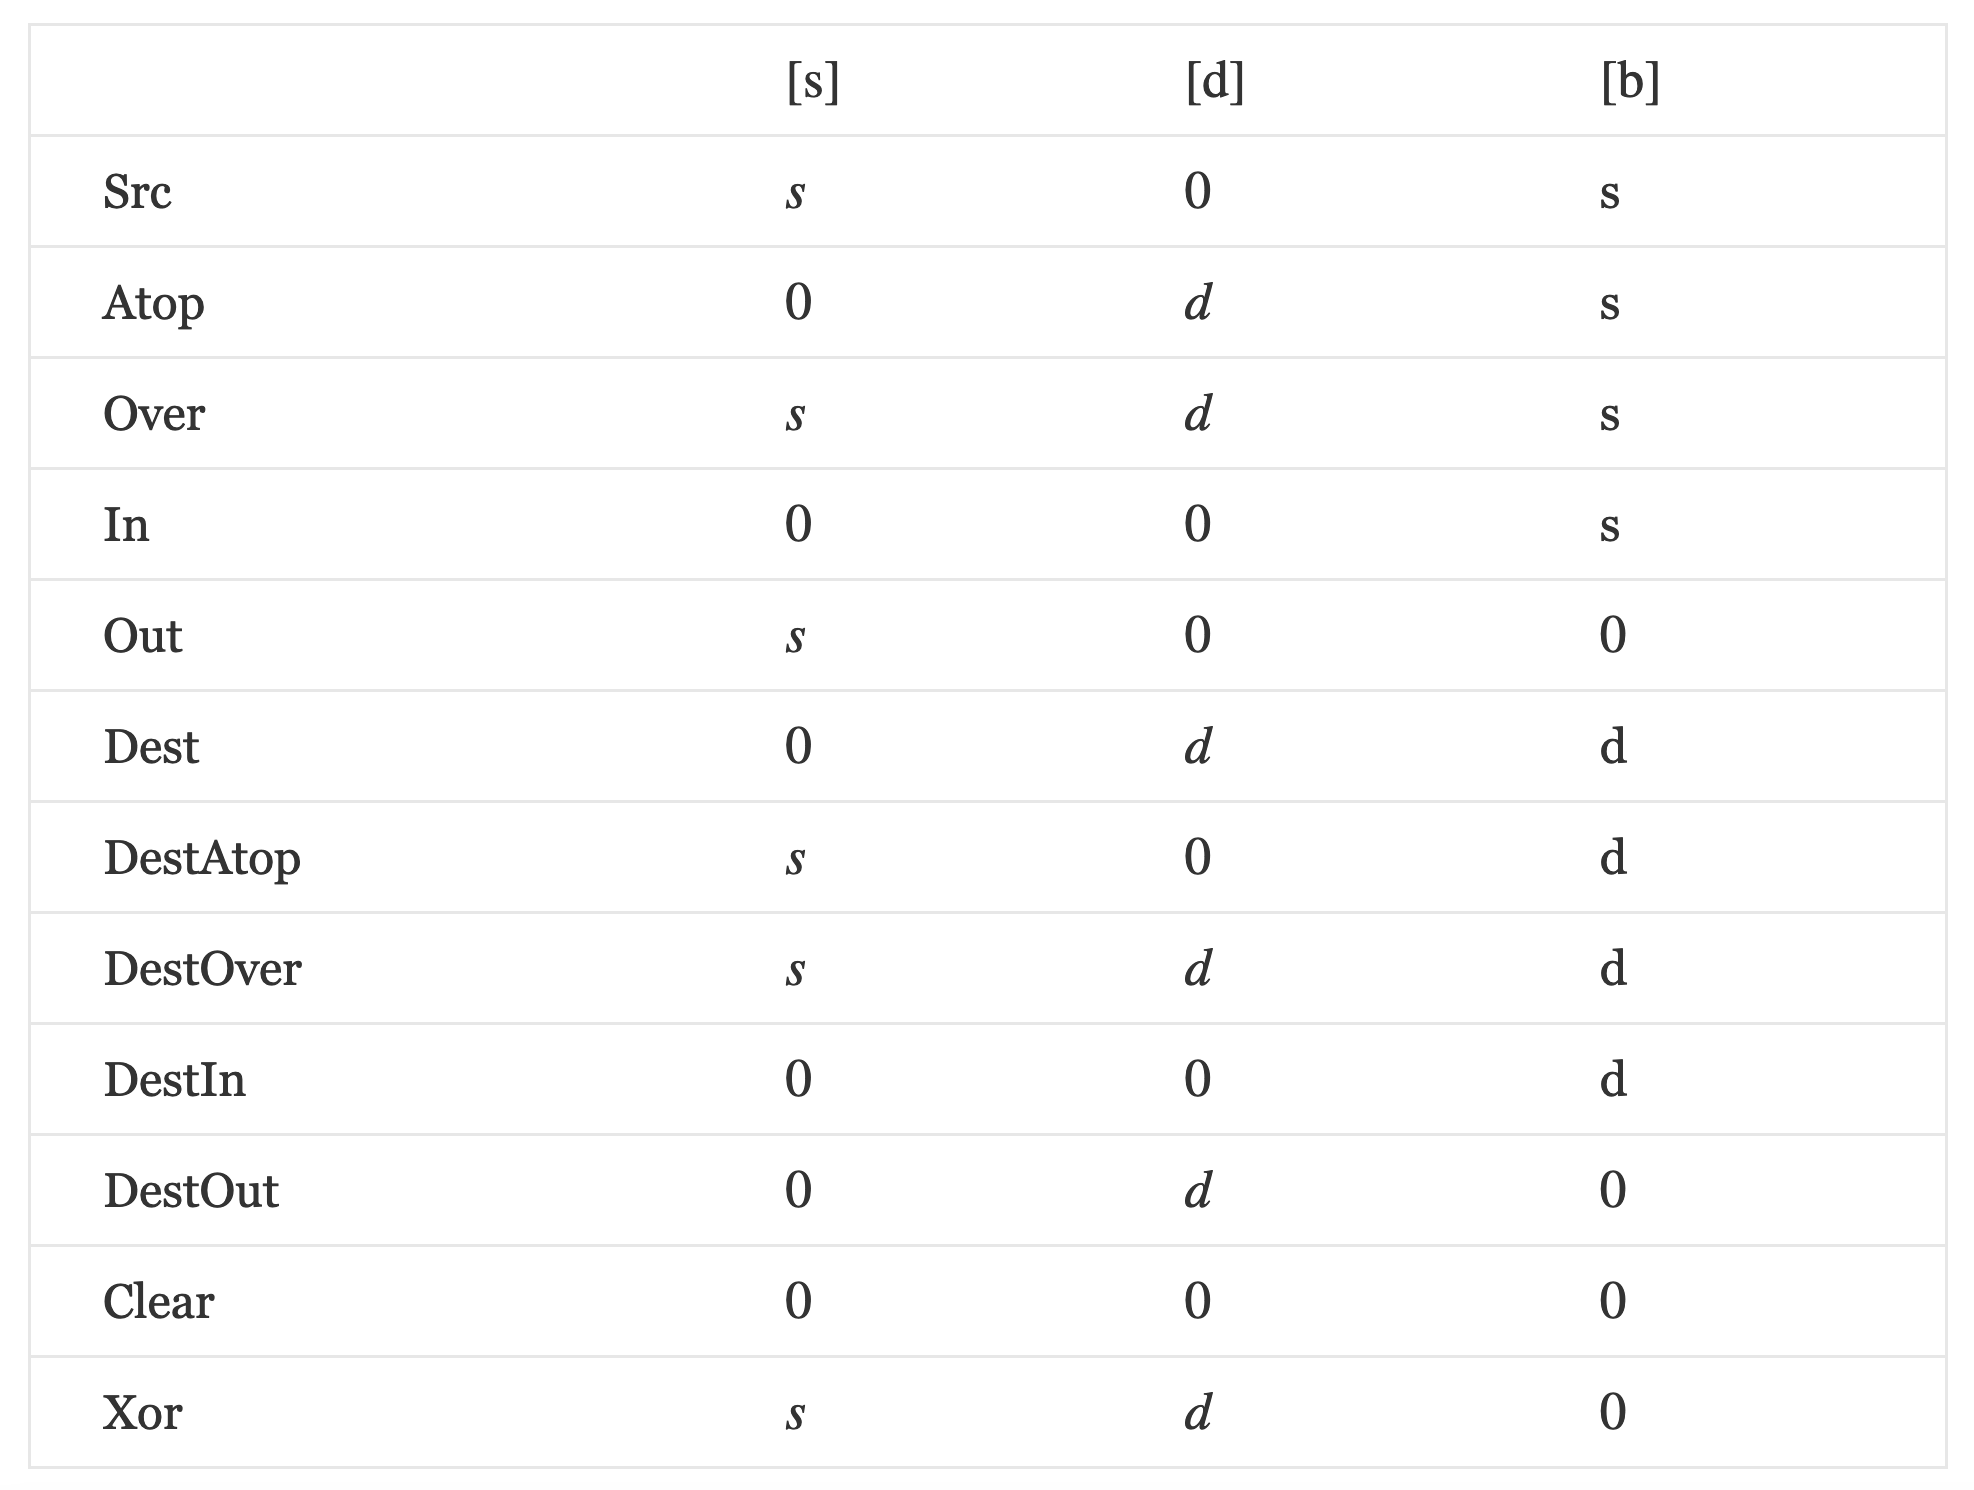
\includegraphics[width=0.7\textwidth]{figs/porter duff}
	\caption{\label{porter duff} Porter/Duff operators table. }
\end{figure}


%%%%%%%%%%%%%%%%%%%%%
% Ray Casting
%%%%%%%%%%%%%%%%%%%%%
\section{Ray Casting} 
In introductory Ray Casting, we consider scenes with no lighting whatsoever, and we consider rays originating from the eye point (camera), through the virtual image plane, and finally hit the objects in the scene. Our goal could be summarized with the following pseudocode, 
\begin{minted}{text}
  for each image pixel {
    generate a ray
    for each scene object { 
      if ray intersects object
        then do something. e.g. set pixel color
    }
  }
\end{minted}

\subsection{Ray}
We introduce the following parametrization of a ray
\begin{equation}
	p(t) = \be + t(\bs - \be)
\end{equation}
where $\be$ is the eye point, $\bs$ is a known point along the path and $p(t)$ is a parametrization of ``point along the ray''. Notice that under our parametrization, we have $p(0) = \be$ and $p(1) = \bs$. 

\subsection{Camera Device}
We consider the simplest ideal pin hole camera, where the pinhole has an infinitesimal size. In real world, this would not be the case. In a real pinhole camera, an aperture is present instead of pinhole. An aperture has a certain (small) size, but it is big enough to cause the image formed become blurry, due to the nature of light. A more complex camera system introduces lens to correct the aperture, i.e. to focus. 

The camera basis could be calculated as follows
\begin{equation}
	\bw = -view, \quad 
	\bu = view \times up, \quad
	\bv = \bw \times \bu
\end{equation}

\subsection{Projection - Orthographic and Perspective}
The most naive ray generation is probably orthographic, where all the rays generated are parallel to each other and they are orthonormal to the image plane. This may sound abstract, but when you draw a cube on paper with parallel edges, you are essentially considering an orthographic projection. 

A more natural looking approach is perspective projection, where rays all originate from the eye point. Each ray will pass through one pixel in the virtual image plane, and finally may or may not intersect an object in the scene. Depending on whether the ray hits an object, different operations are done to the manipulate the resulting image. 

\subsubsection{Transforming Between Coordinate Systems}
\begin{figure}
	\center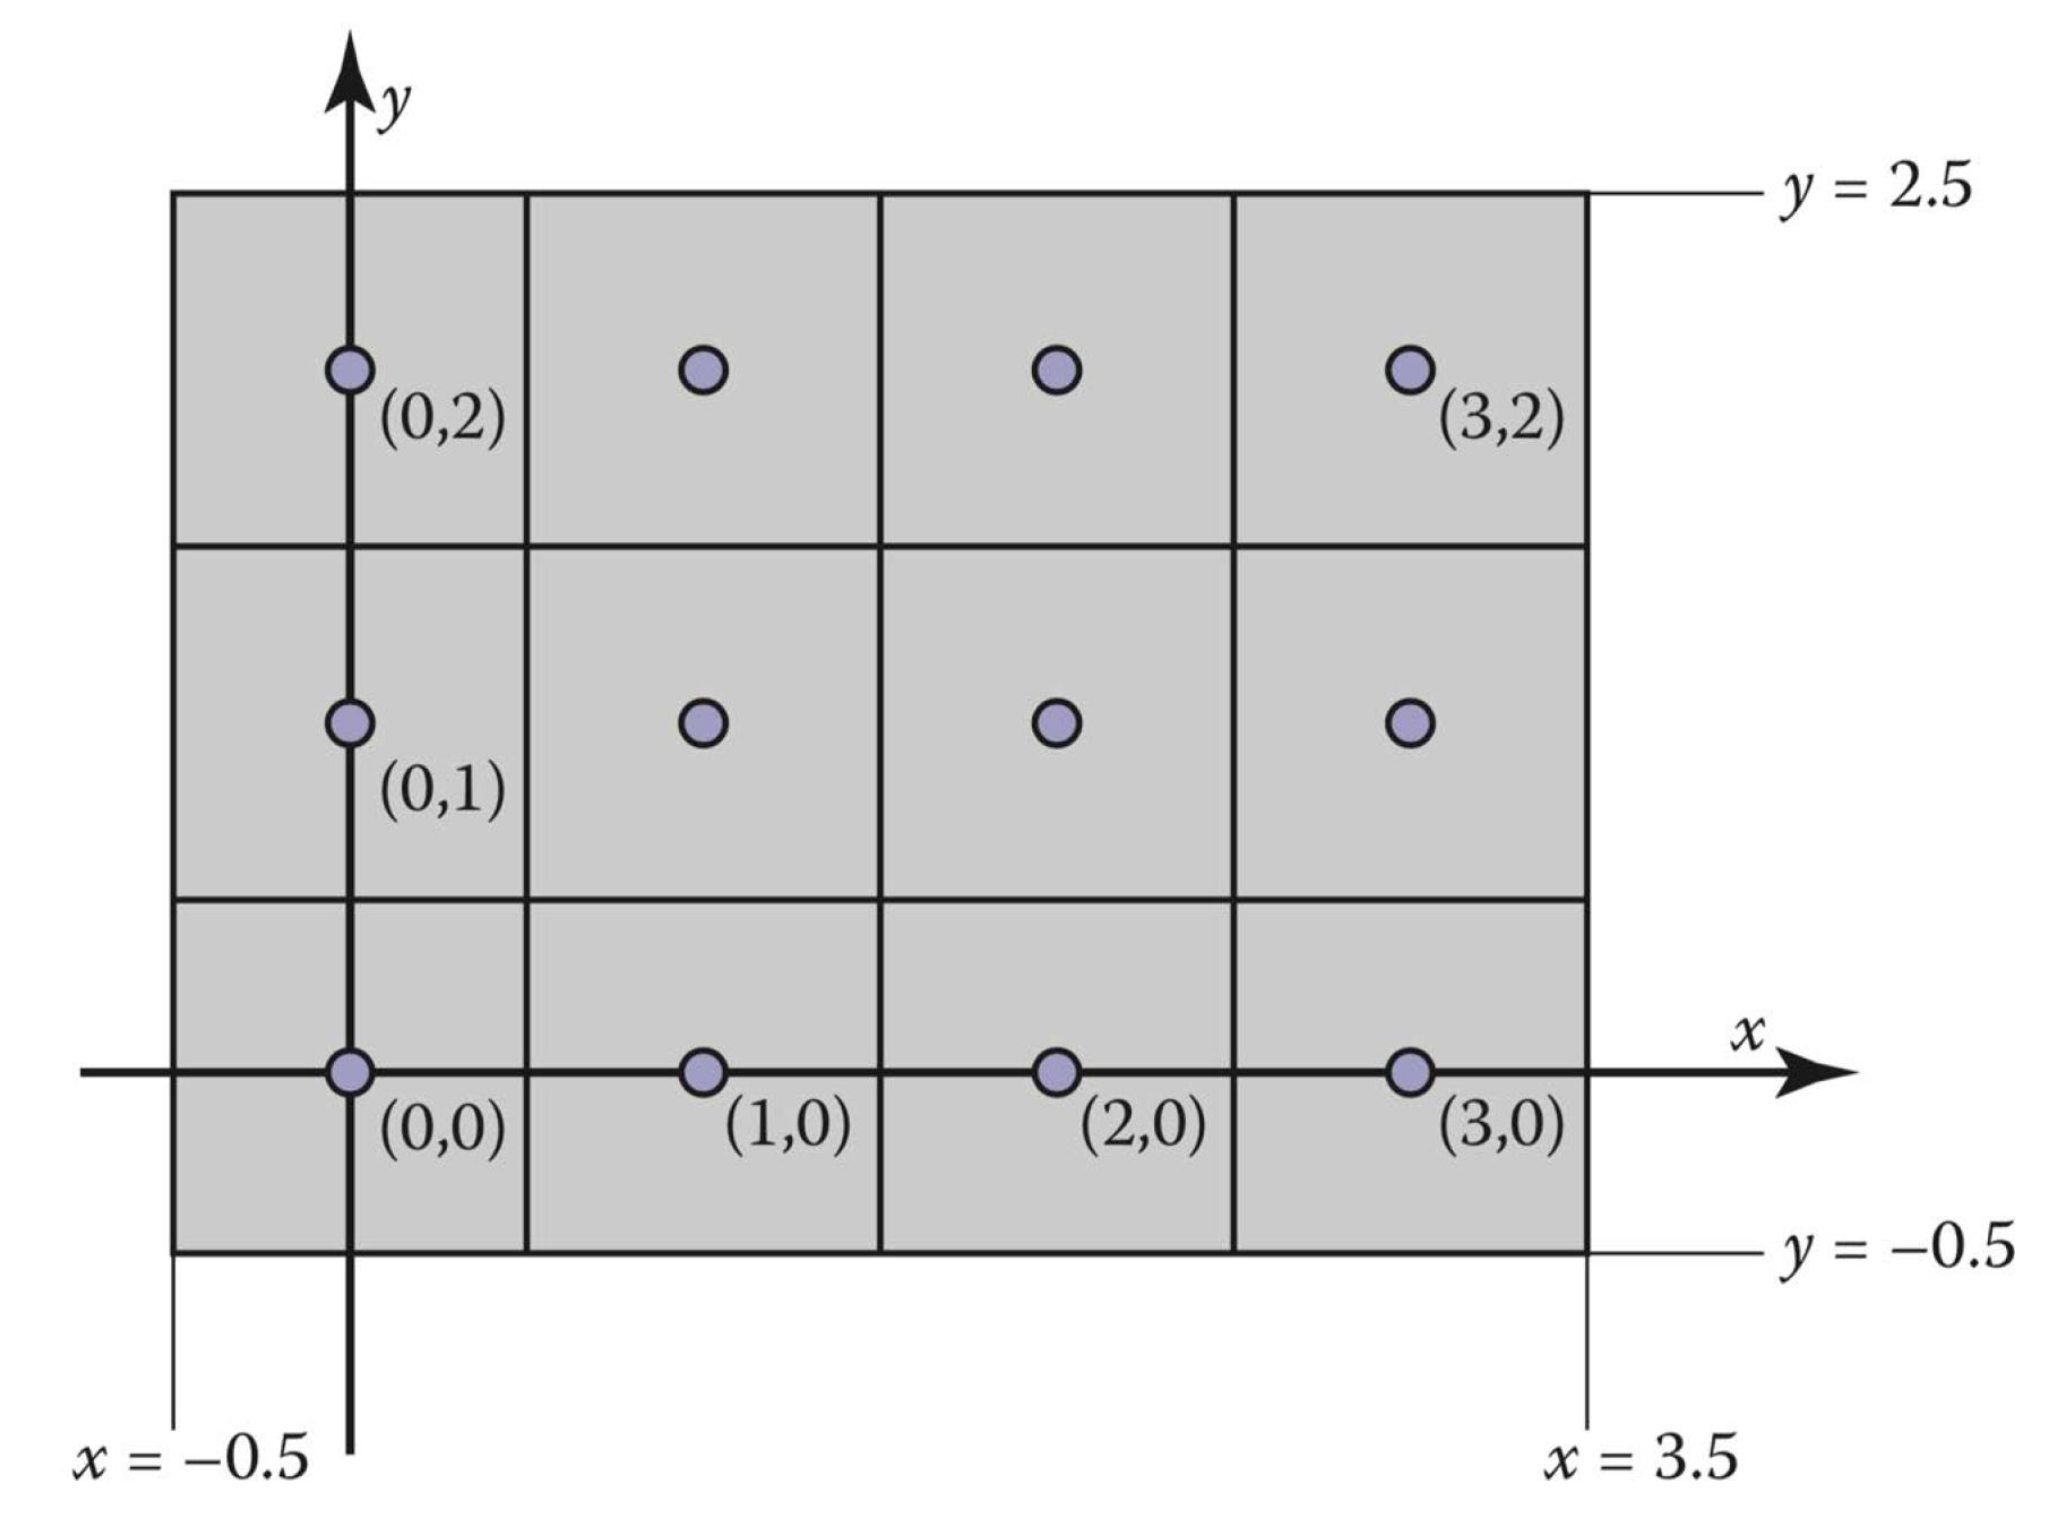
\includegraphics[width=0.7\textwidth]{figs/standard pixel coordinate systems}
	\caption{\label{fig:standard pixel coordinate system} The Standard Pixel Coordinate System. }
\end{figure}
Figure \ref{fig:standard pixel coordinate system} shows the standard pixel coordinate system, where the centre of the bottom left corner pixel is marked as the origin, $(0, 0)$. We will need to handle this subtlety when casting rays. 

Consider $n_x, n_y$ to be the number of pixels on $X$ and $Y$ directions respectively, and $width, height$ to be the physical width and height of the image (size of image plane). Then, 
\begin{itemize}
	\item Bottom left corner (pixel space) is $(-1/2, -1/2)$,
	\item Top right corner (pixel space) is $(n_x - 1/2, n_y - 1/2)$, 
	\item Bottom left corner (camera space) is $(-width / 2, -height / 2)$, 
	\item Top right corner (camera space) is $(width / 2, height / 2)$
\end{itemize}
Do notice in the camera space, if we start at the position at the camera, and move in the direction of $view$ ($-\bw$) then we shall arrive at the centre of the image plane, rather than any corner. Solving the above, we know that pixel at position $(i, j)$ in the raster image has the position $(u, v)$ where
\begin{equation}
	u = \frac{width}{n_x} \left( i + \frac{1}{2} \right) - \frac{width}{2} \label{eq:u transform}
\end{equation}
and 
\begin{equation}
	v = \frac{height}{n_y} \left( j + \frac{1}{2} \right) - \frac{height}{2} \label{eq:v transform}
\end{equation}

\subsection{Ray Equations}
\subsubsection{... in Camera Space}
We previously stated that the ray equation should have the form 
\begin{equation}
	\bp(t) = \be + t(\bs - \be)
\end{equation}
In camera space, we will be at the starting point of the ray, which means that the eye point is exactly origin. Substituting this information into the equation, we have
\begin{equation}
	\mathbf{p}(t)=\left[\begin{array}{l}
		0 \\
		0 \\
		0
		\end{array}\right]+t\left(\left[\begin{array}{l}
		u(i) \\
		v(j) \\
		-d
		\end{array}\right]-\left[\begin{array}{l}
		0 \\
		0 \\
		0
	\end{array}\right]\right) = t\begin{bmatrix}
		u(i) \\ v(j) \\ -d
	\end{bmatrix}
\end{equation}
where $d$ is the length between the eye point and the image plane, commonly known as focal length. And $u, v$ calculated using Equations \ref{eq:u transform} and \ref{eq:v transform}. 

\subsubsection{... in World Space}
The world space representation could be attained using a change of coordinates, 
\begin{equation}
	\mathbf{p}(t)=\mathbf{e}+t(u(i) \mathbf{u}+v(j) \mathbf{v}+-d \mathbf{w}) 
\end{equation}
which could be written in matrix form 
\begin{equation}
	\bp(t) = \be + t \begin{bmatrix}
		\bu & \bv & \bw
	\end{bmatrix}_{M_{3 \times 3}(\real)} \begin{bmatrix}
		u(i) \\ v(j) \\-d
	\end{bmatrix}
\end{equation}
where the 3-by-3 matrix in the middle is called the Camera Transformation Matrix, and rest elements calculated as previous. 

\subsection{Intersection Tests}
Now that we have discussed how to generate a ray and how to get the ray in different representations, it is time to move to the \texttt{if} statement in our pseudo code, which was to check if an intersection exists between a ray and a scene object. 
\subsubsection{Ray-Plane Intersection}
A plane is defined by the equation ($\bq$ such that satisfies the following)
\begin{equation}
	\bn \cdot ( \bq - \bp_0) = 0
\end{equation}
where $\bn$ is the surface normal and $\bp_0$ is a point on the surface. To see if a ray intersects with a plane, it suffices to substitute $\bp$ with the parametrized ray equation, and try to solve for $t$, i.e. we want to solve for $t$ in
\begin{equation}
	\bn \cdot ((\be + t\bd) - \bp_0) = 0
\end{equation}
where $\bd$ is the ray direction, equal to $\bs - \be$. Solving the above yields
\begin{equation}
	t = \frac{-\bn \cdot ( \be - \bp_0)}{\bn \cdot \bd}
\end{equation}
Notice that the intersection exists iff $t \in \real$, in particular if $\bn$ and $\bd$ are collinear, then $t$ would blow up. In practice, it is usually useful to do the checking first, to avoid numeric issues. 

\subsubsection{Ray-Sphere Intersection}
We use an implicit equation to define a sphere that is centred at $\bc$ with radius $r$ ($\bq$ such that satisfies the following)
\begin{equation}
	(\bq - \bc) \cdot (\bq - \bc) - r^2 = 0
\end{equation}
Again, we substitute $\bq$ with the ray parametrization, 
\begin{equation}
	(\be + t \bd - \bc ) \cdot (\be + t \bd - \bc ) - r^2 = 0 
\end{equation}
expanding and rearranging yields
\begin{equation}
	(\bd \cdot \bd) t^2 + 2\bd \cdot (\be - \bc) t + (\be - \bc) \cdot (\be - \bc) - r^2 = 0
\end{equation}
To solve this, we can resort to the quadratic equation. First we calculate the discriminant, 
\begin{equation}
	\Delta = (2\bd \cdot (\be - \bc)) ^2 - 4(\bd \cdot \bd)((\be - \bc) \cdot (\be - \bc) - r^2)
\end{equation}
Clearly, if $\Delta < 0$ then there is no intersection. If $\Delta = 0$ then the ray is tangential to the sphere, and the ray has two intersection points with the sphere otherwise. The exact solution(s) could be calculated as 
\begin{equation}
	t = \frac{-2\bd\cdot(\be - \bc) \pm \sqrt{\Delta}}{2\bd \cdot \bd}
\end{equation}

\subsubsection{Ray-Triangle Intersection}
In this case, we parametrized a triangle as 
\begin{equation}
	\bq = \bp_0 + \alpha \bt_1 + \beta \bt_2
\end{equation}
where $\bp_0$ is a vertex of the triangle and $\bt_1, \bt_2$ are two edges shooting outwards from $\bp_0$. In order to make this a triangle, there are several constraints, namely
\begin{equation}
	\alpha \geq 0, \quad \beta \geq 0, \quad \alpha + \beta \leq 1.
\end{equation}

%%%%%%%%%%%%%%%%%%%%%
% Ray Tracing
%%%%%%%%%%%%%%%%%%%%%
\section{Ray Tracing}
\subsection{Light and Surfaces}
There are two types of lights, namely directional and point light sources. 
\begin{itemize}
	\item The directional light has its light direction independent of the object, this typically happens when the light is very far away. (e.g. the sun)
	\item On the other hand, point light are such that the direction of light depends on position of object relative to light. Think of this as a light bulb in a room. 
\end{itemize}
\subsection{Shading}
The goal of shading is to compute the light reflected toward camera. As an algorithm it expects the following inputs: eye direction, light direction for each of many lights, surface normal, and surface parameters such as color and shininess. 

\paragraph{The Surface Normal} at a hit point can be computed, depending on the type of specification
\begin{itemize}
	\item Polygon normal: cross product of two non-collinear edges, 
	\item Implicit surface normal $f(p) = 0$: $gradient(f)(p)$
	\item Explicit parametric surface $f(a,b)$: 
	\begin{equation}
		\frac{\partial f(s, b)}{\partial s} \times \frac{\partial f(a, t)}{\partial t}
	\end{equation}
\end{itemize}

\subsection{Light Falloff}
The light falloff aims to model the concept of diminishing light intensity based on distance. Suppose the light source has intensity of $I$, then, at a point that is $r$ (Euclidean Distance) away from the light source, the light intensity from that particular light source would be
\begin{equation}
	\text{Intensity}(I, r) = I / r^2
\end{equation}
Clearly, when we are at the light source, $r = 0$ and we attain the max intensity. 

\subsection{Diffuse Reflection}
In the case of diffuse reflection, light are scattered uniformly in all directions, i.e. he surface color is the same for all viewing directions. The amount of light captured by a surface obeys Lamber's cosine law. (We call this Lambertian surface.) Figure \ref{lambert} illustrates the relationship. 

\begin{figure}
	\centering 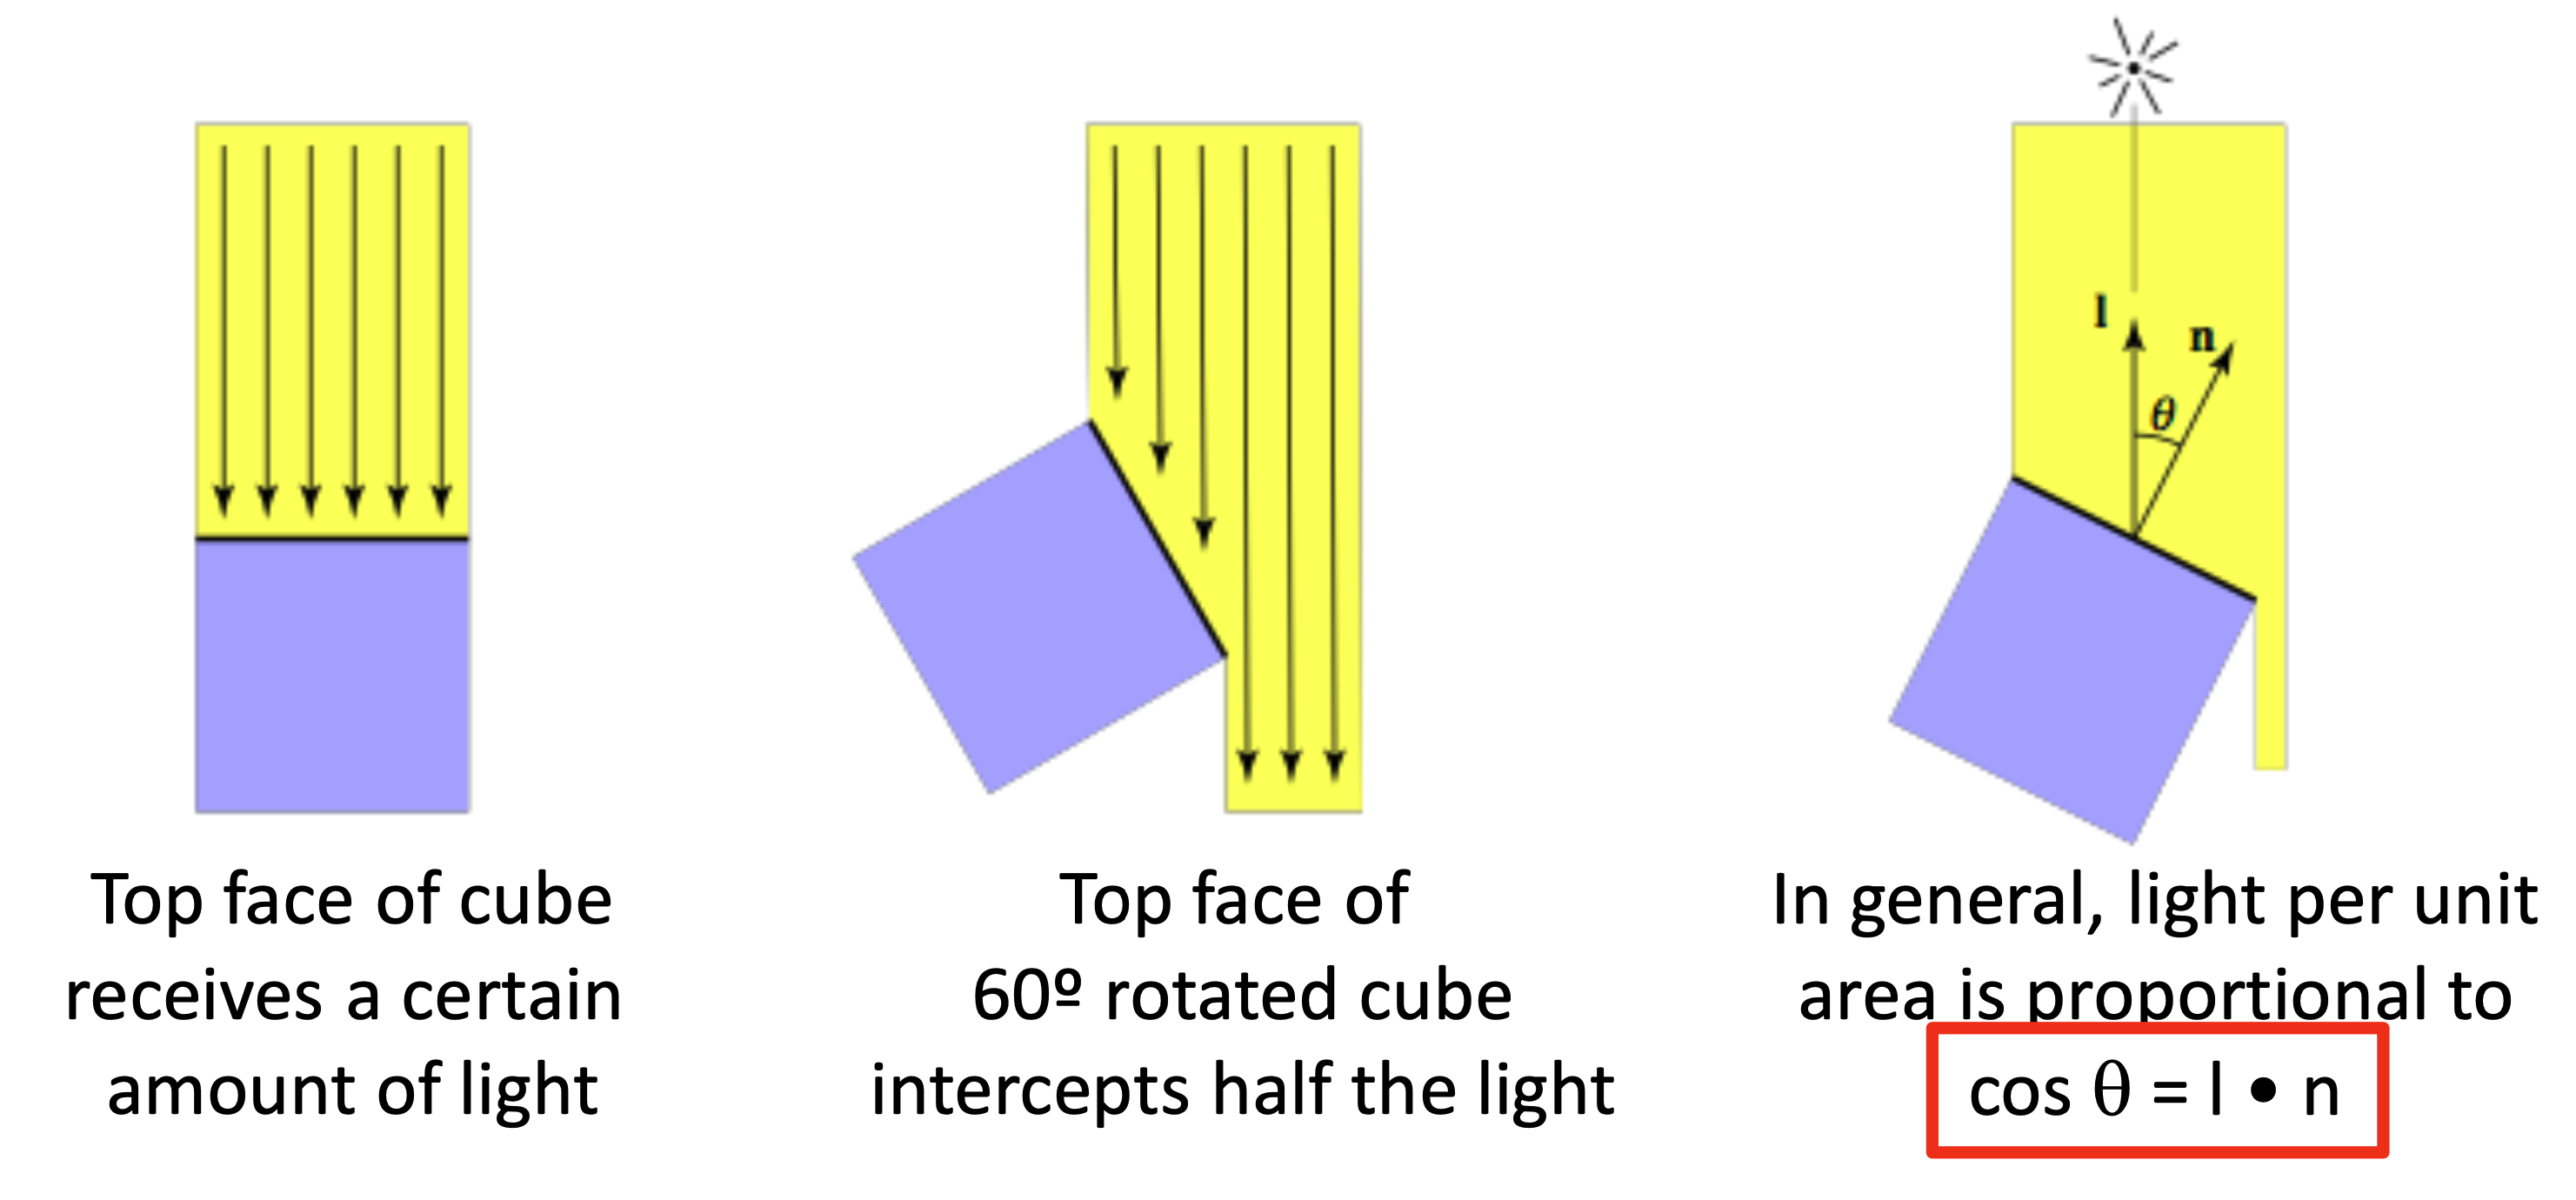
\includegraphics[width=0.7\textwidth]{figs/lambert}
	\caption{\label{lambert} Illustration of Lambert's cosine law. }
\end{figure}

\subsection{Lambertian Shading} 
The Lambertian Shading is independent of view direction. Let's call $L_d:=$ diffusely reflected light, $k_d:=$ diffuse coefficient\note{$k_d$ could be separate for three color channels. }, and $I:=$ illumination from source, then 
\begin{equation}
	L_{d}=k_{d}\circ \left(I / r^{2}\right) \max (0, \mathbf{n} \cdot \mathbf{l})
\end{equation}
This produces a matte appearance. 

\subsection{Shadows}
Surface is only illuminated if nothing blocks its view of the light. With ray tracing it's easy to check if a point in the scene is in shadow, all you have to do is just shoot a ray from the point\footnote{This ``point'' means the actual location in 3d of what a pixel on the image projects to. } to the light and intersect it with the scene.

\subsection{Multiple Light Sources}
\begin{itemize}
	\item Important to fill in black shadows, 
	\item and just loop over lights, add contributions
	\item Ambient shading
	\begin{itemize}
		\item Black shadows are not really right, 
		\item easy solution: dim light at the camera, so everything we see must  be lit up (might be dim, but not black)
		\item alternative: add a constant ambient color to the shading. 
	\end{itemize}
\end{itemize}

\subsection{Ambient Shading}
Ambient shading are those that does not depend on anything, we add a constant color to account for disregarded illumination and fill in black shadows. Let's call $L_a:=$ reflected ambient light, $k_a:=$ ambient coefficient\note{This $k_a$ could again be separate for different color channels}, and $I_a$ the raw light intensity, then
\begin{equation}
	L_a = k_a \circ I_a
\end{equation}

\subsection{Algorithm Template}
Let's present the algorithm template for images with multiple light sources here
\begin{mdframed}
	\begin{minted}{cpp}
shade(ray, lights, point, normal) {
    result = ambient; 
    for light in lights {
        I = light.pos - position; 
        shadowray = (point + eps * normal, I); 
        if !scene.intersection(result, shadowray) {
            it = surface.k * light.intensity * max(0, normal.dot(I));
            result += surface.color * it;
        }
    }
    return result; 
}
	\end{minted}
\end{mdframed}
Do notice that we have \texttt{shadowray = (point + eps * normal, I);}, and the eps is there to prevent floating point numerical errors. If we don't do that it is possible a ray would intersect immediately with the surface, and produce unusable images. 

\subsection{Mirror Reflection}
Now we've talked about diffuse reflections (matte surfaces), let's see the case of mirror reflection. We discuss the case of imperfect mirror here, where the intensity depends on view direction - reflects incident light from mirror direction. Figure \ref{mirror reflection} illustrates the scenario. The reflected ray vector is 
\begin{equation}
	\br = 2 (\bn \cdot \bl) \bn - \bl
\end{equation}
\begin{figure}
	\centering 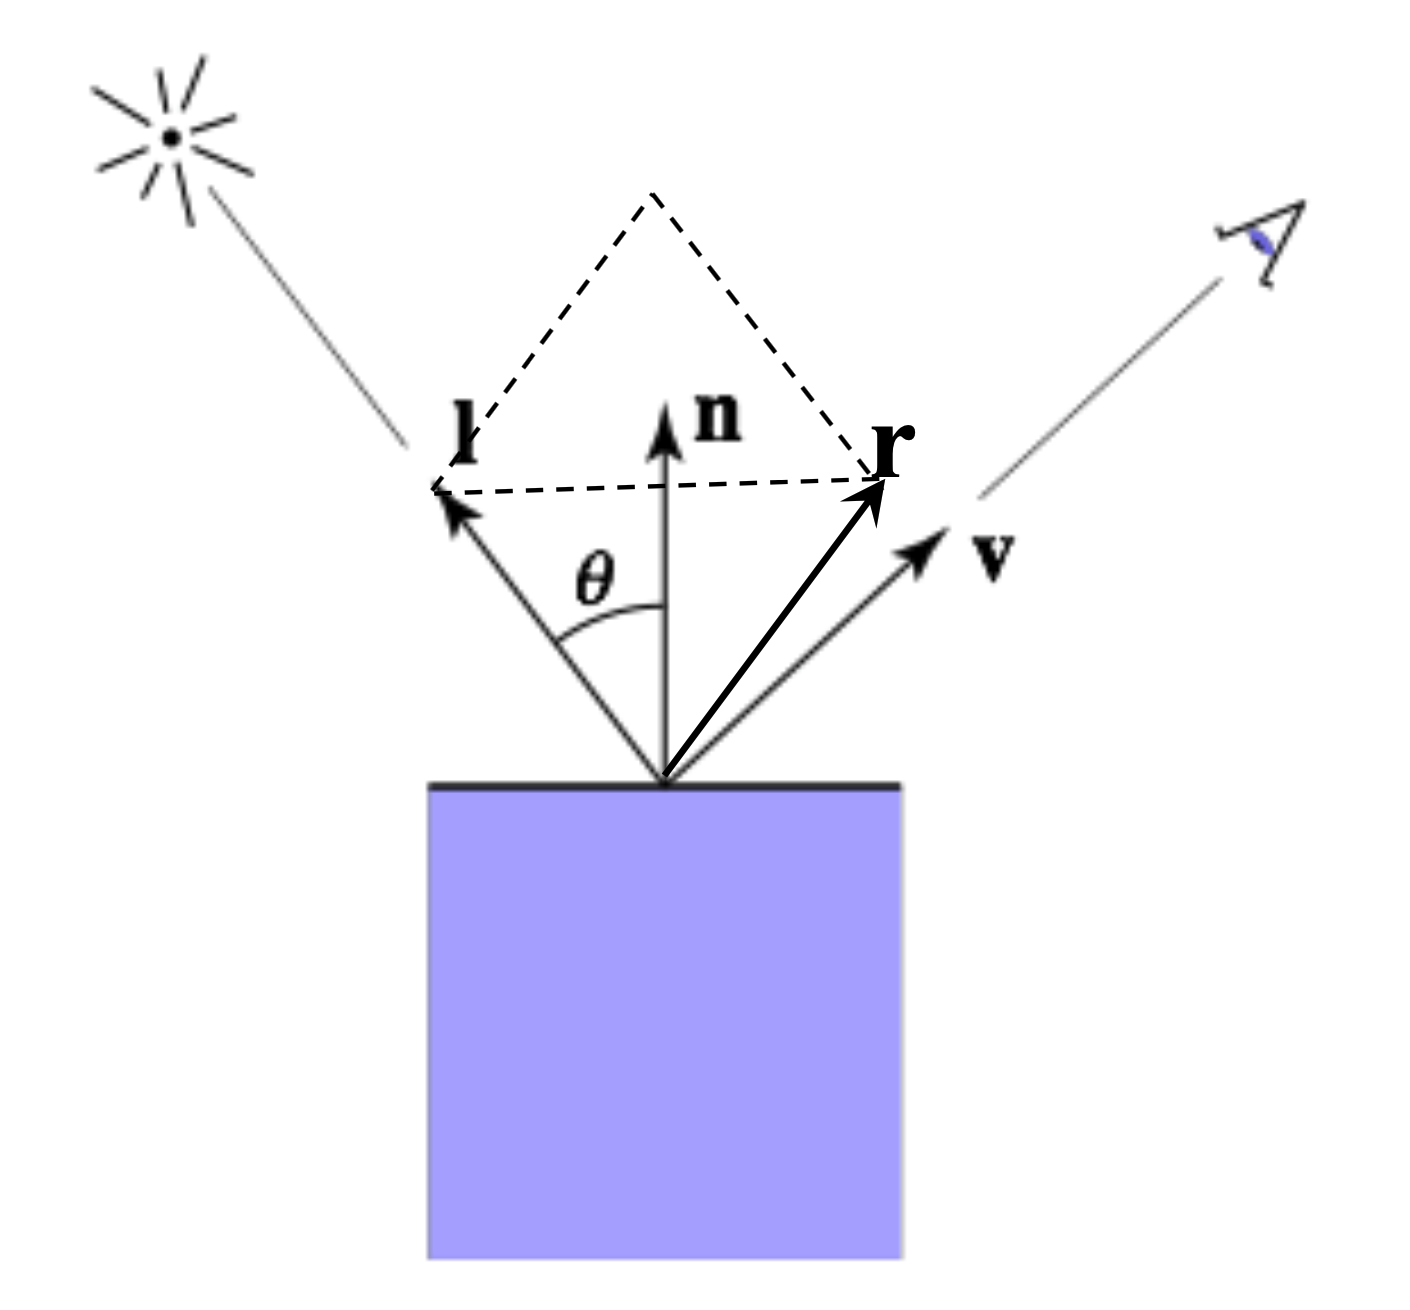
\includegraphics[width=0.5\textwidth]{figs/mirror reflection}
	\caption{\label{mirror reflection} Mirror reflection illustration}
\end{figure}

\subsection{Phong Specular Shading}
With a perfect mirror, only when $\br = \bv$ in Figure \ref{mirror reflection} would the eye see light. In real world, this rarely is the case and we wish to model a common imperfect mirror where there will be some light being reflected to directions around $\br$. Phong specular shading aims to model reflections from this imperfect mirror - the intensity would depend on the view direction, and is bright near mirror configuration: 
\begin{equation}
	k_s \circ I_s (\bv \cdot \br)^{shiny}
\end{equation}
where $k_s$ is yet another set of coefficient guarding three channels, $I_s$ is the three channel intensity (distance decay taken into account already), and $shiny$ is a constant hyper-parameter raised to exponent dictating how fast the $(\bv \cdot \br)$ diminishes to $0$. A large $shiny$ exponent will make the surface more glossy, while a smaller one will make the surface more matte-looking. 

\subsection{Blinn(-Phong) Specular Shading}
Blinn specular shading is just another formulation.\footnote{This very simple and widely used model for specular highlights was proposed by Phong (Phong, 1975) and later updated by Blinn (J. F. Blinn, 1976) to the form most commonly used today.} Figure \ref{blinn} illustrate what we want to calculate. Let's call the point of reflection $\bo$, then in Phong model, we used $angle\br\bo\bv$ to model the angle and here in Blinn we will be using $\angle\bh\bo\bn$ instead. Notice that however, we do need to calculate an extra vector $\bh$ that is the normalized sum of $\bv$ and $\bl$, i.e. 
\begin{equation}
	\mathbf{h}=\frac{\mathbf{v}+\bl}{\|\mathbf{v}+\bl\|}
\end{equation}
The specular reflected intensities can be calculated
\begin{equation}ci
	L = k_s \circ I \max \{ 0, \bn \cdot \bh \}^p
\end{equation}
where $k_s$ is our guarding coefficients, $I$ is the intensity at the point of reflection (distance decay taken into account already), $p$ is something similar to $shiny$ from before. Again, a larger $p$ means a shinier surface and  a smaller one means more matte-looking. 

\begin{figure}
	\centering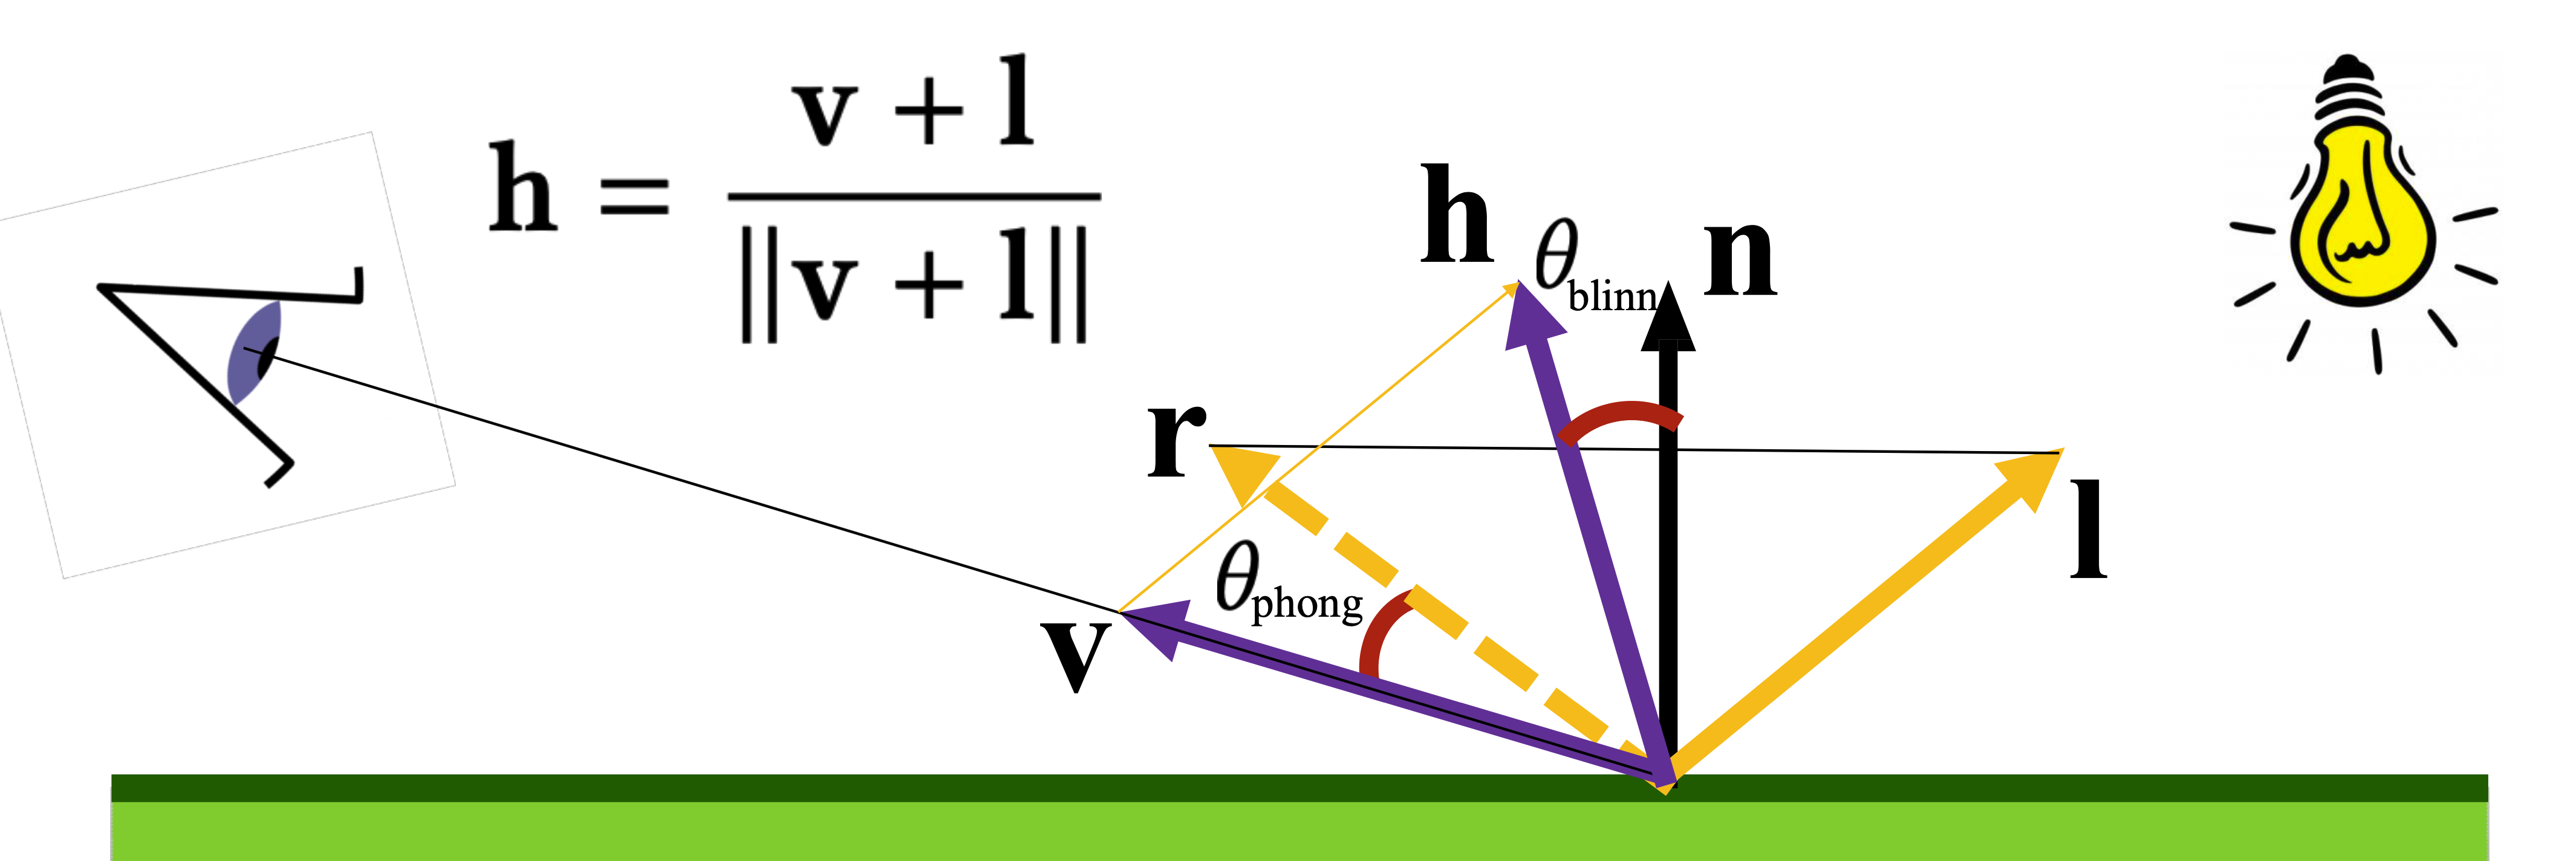
\includegraphics[width=0.8\textwidth]{figs/blinn}
	\caption{\label{blinn} Blinn Specular Shading and Phong Specular Shading.}
\end{figure}

\subsection{Local Illumination}
\begin{itemize}
	\item Usually include ambient, diffuse, Blinn-Phong in one model
	\begin{equation}
		\begin{aligned}
			L &=L_{a}+L_{d}+L_{s} \\
			&=k_{a} I_{a}+k_{d}\left(I / r^{2}\right) \max (0, \mathbf{n} \cdot \mathbf{l})+k_{s}\left(I / r^{2}\right) \max (0, \mathbf{n} \cdot \mathbf{h})^{p}
		\end{aligned}
	\end{equation}
	\item The final result is the sum over many lights
	\begin{align}
		L
		&= L_{a}+\sum_{i=1}^{N}\left[\left(L_{d}\right)_{i}+\left(L_{s}\right)_{i}\right] \\
		&=k_{a} I_{a}+\sum_{i=1}^{N}\left[k_{d}\left(I_{i} / r_{i}^{2}\right) \max \left(0, \mathbf{n} \cdot \mathbf{l}_{i}\right)+
		k_{s}\left(I_{i} / r_{i}^{2}\right) \max \left(0, \mathbf{n} \cdot \mathbf{h}_{i}\right)^{p}\right]
	\end{align}
\end{itemize}

\subsection{Ray Tracing Template}
{\center 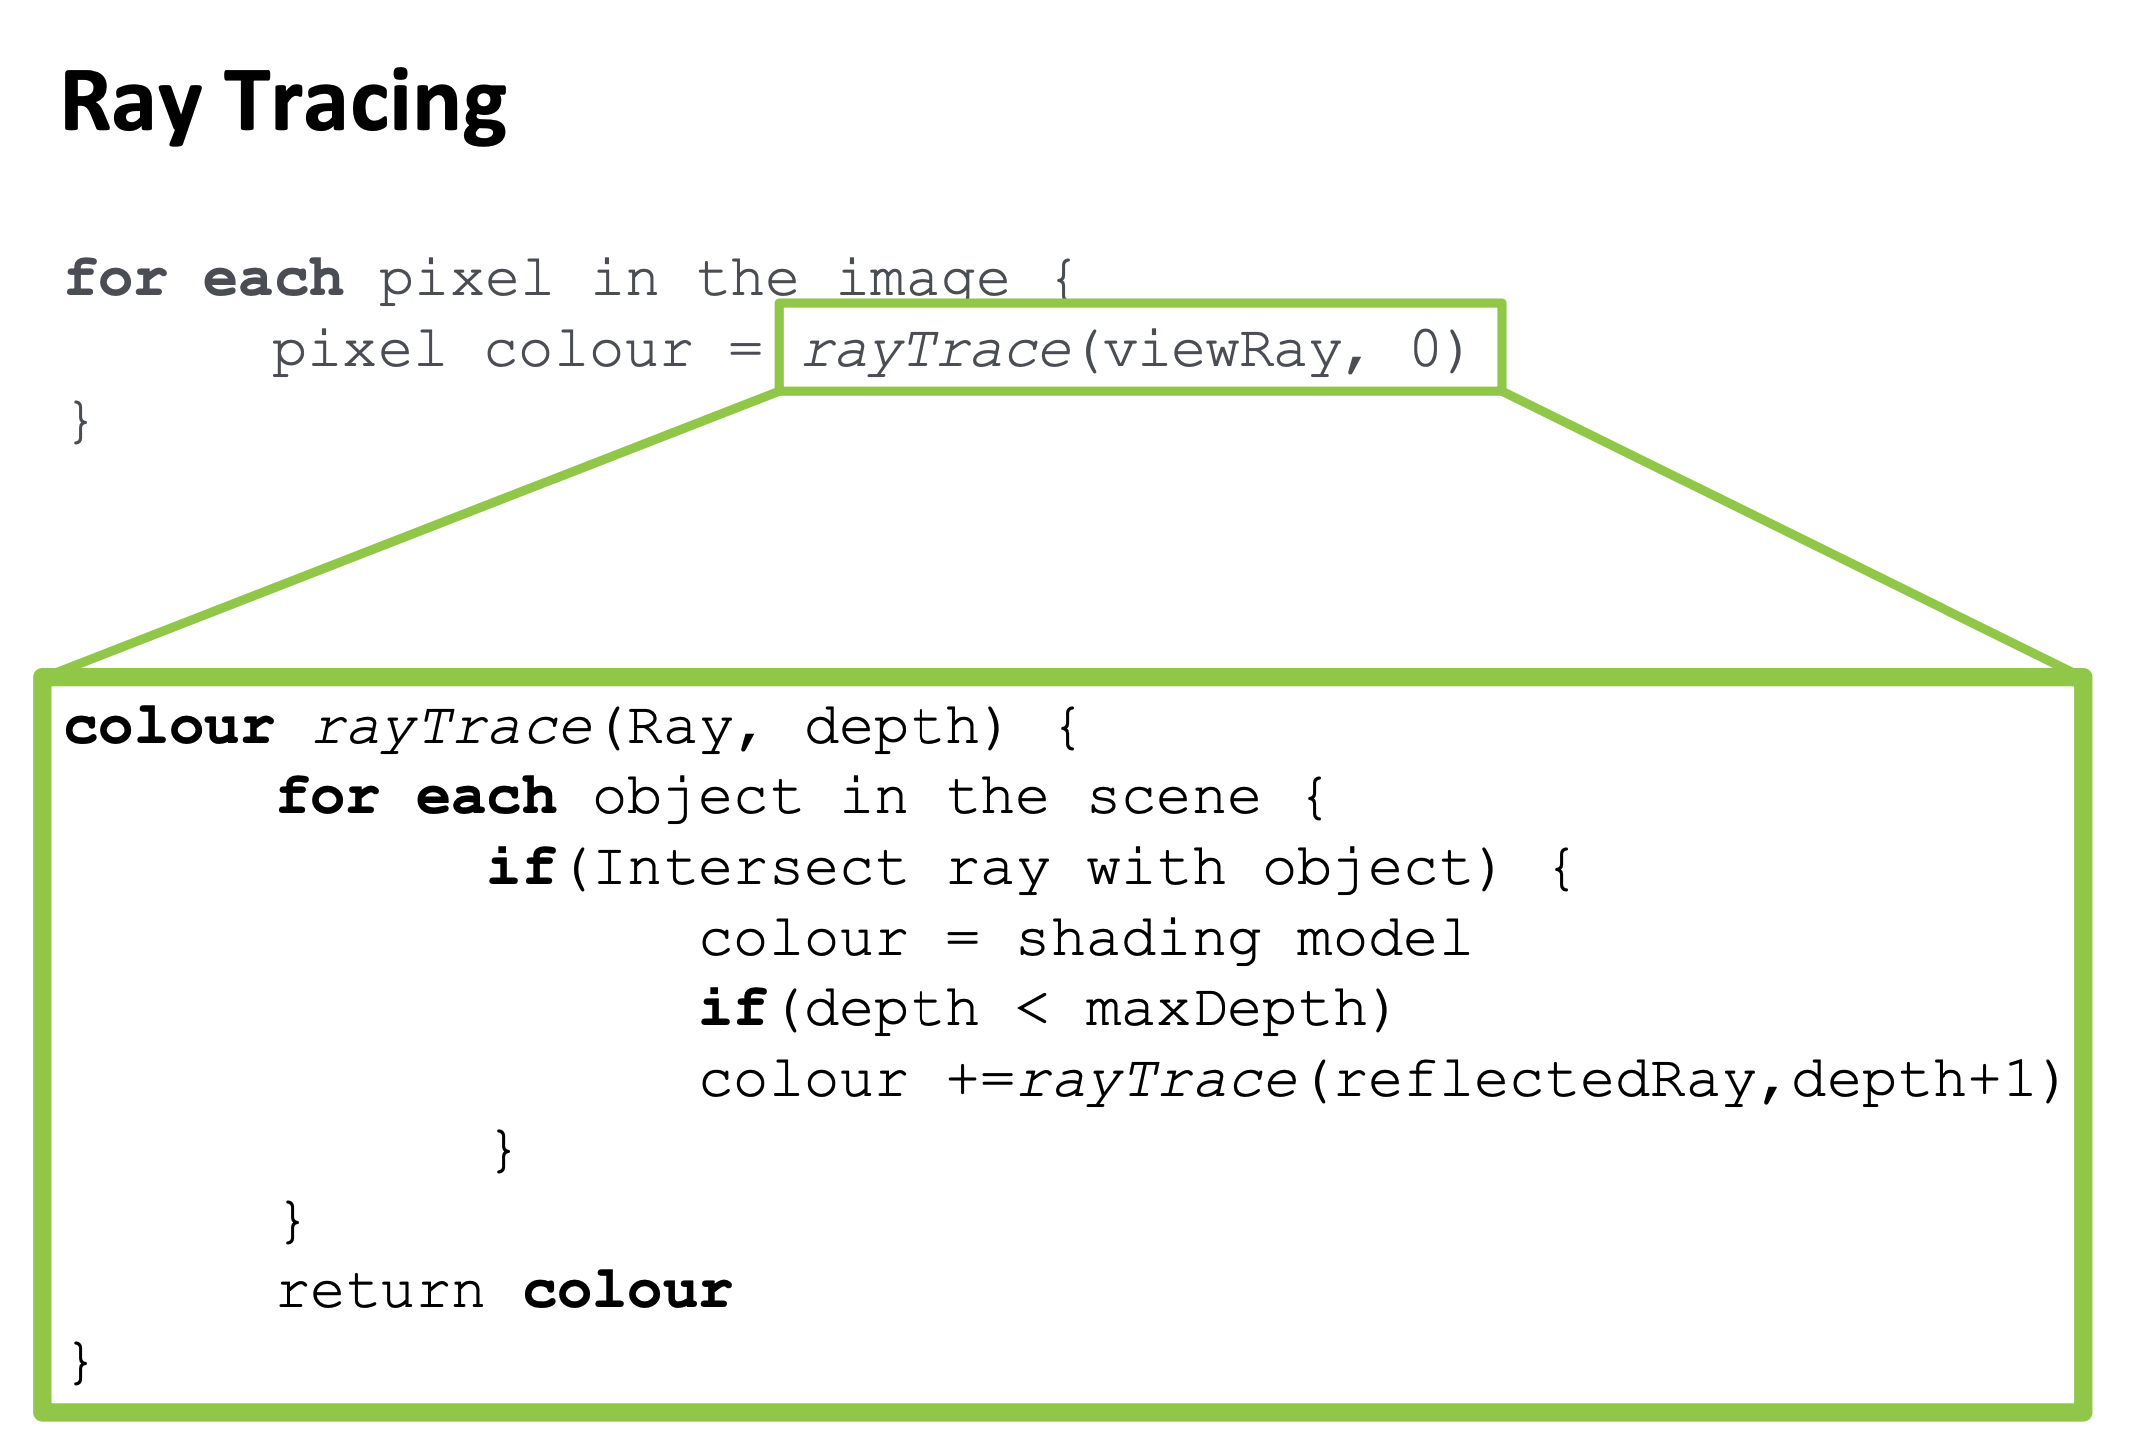
\includegraphics[width=1.0\textwidth]{figs/ray trace}}

\subsection{Refraction - Snell's Law}
Consider a surface with normal $\bn$, with incoming light vector $-\bl$ (so $\bl$ is pointing into the surface), call $\theta_l := \angle\bn\bo\bl$. Suppose the refracted light vector is named $\bt$ with $\theta_t:= \angle \bt\bo (-\bn )$, then Snell's Law states that
\begin{equation}
	c_l \sin\theta_l = c_t \sin \theta_t
\end{equation}
We can derive that our unknown of interest $\bt$ is such that 
\begin{equation}
	\bt = -\frac{c_l}{c_t}\bl + \frac{c_l}{c_t} \cos(\theta_l) \bn - \cos (\theta_t ) \bn
\end{equation}
To take refractions into account, we just need to slightly modify the ray tracing template presented previously. Namely, we will need to add 
\begin{verbatim}
	...
	colour += raytrace(reflectedRay, depth+1)
	colour += raytrace(refractedRay, depth+1)
\end{verbatim}

\subsection{Ray Tracing: Pros and Cons}
Ray tracing provides a unifying framework for all of the following
\begin{itemize}
	\item Hidden surface removal, 
	\item shadow computation, 
	\item reflection of light, 
	\item refraction of light, 
	\item globular specular interaction 
\end{itemize}
but at the same time it presents some deficiencies
\begin{itemize}
	\item intersection computation time can be long, (solution: bounding volumes, next time)
	\item recursive algorithm can lead to exponential complexity, (solution: stochastic sampling)
	\item ignores light transport mechanisms involving diffuse surfaces. 
\end{itemize}

\subsection{Caustics}
\subsection{Radiosity}
\subsection{The Rending Equation}
\begin{equation}
	L_{o}(\bx, \bw)
	=
	L_{e}(\bx, \bw) 
	+
	\int_{\Omega} f_{r}\left(\bx, \bw^{\prime}, \bw\right) L_{i}\left(\bx, \bw^{\prime}\right)\left(\bw^{\prime} \cdot \bn\right) \mathrm{d} \bw^{\prime}
\end{equation}
where 
\begin{align}
	&L_{o}(x, \vec{w}) = \text{outgoing light at $\bx$ direction $\bw$} \\
	&L_{e}(x, \vec{w}) = \text{emitted light at position $\bx$ and direction $\bw$} \\
	&\int_\Omega \dots \mathrm d \bw = \text{reflected light at position $\bx$ and direction $\bw$}
\end{align}
where 
\begin{align}
	&f_{r}\left(\bx, \bw^{\prime}, \bw\right) 
	= \text{BRDF: a function describing how light is reflected at an opaque surface} \\
	&L_{i}\left(\bx, \bw^{\prime}\right) 
	= \text{the incoming light from all directions}
\end{align}
\subsection{Soft Light}


%%%%%%%%%%%%%%%%%%%%%
% BVH - AABB
%%%%%%%%%%%%%%%%%%%%%
\section{Spatial Data Structures - Bounding Volume Hierarchy}
In many applications of computer graphics, it is crucial that we can quickly perform queries on a set scene. However, the brute force solution may turn out to be computationally too costly. In a remedy to this problem, we introduce the idea of spatial data structures. These structures partition spaces into smaller ones: (following characterizations are from the text book (Shirley, P., \& Marschner, S., 2009).)
\begin{itemize}
	\item Structures that group objects together into a hierarchy are object partitioning schemes: objects are divided into disjoint groups, but the groups may end up overlapping in space.
	\item Structures that divide space into disjoint regions are space partitioning schemes: space is divided into separate partitions, but one object may have to intersect more than one partition.
	\item Space partitioning schemes can be regular, in which space is divided into uniformly shaped pieces, or irregular, in which space is divided adaptively into irregular pieces, with smaller pieces where there are more and smaller objects.
\end{itemize}

\subsection{(Axis Aligned) Bounding Boxes}
To derive, let's start with the 2D case. Suppose we have a bounding box described by four lines, 
\begin{align}
	x &= x_{\min}, &\text{the lower horizontal line}, \\
	x &= x_{\max}, &\text{the upper horizontal line}, \\
	y &= y_{\min}, &\text{the left vertical line}, \\
	y &= y_{\max}, &\text{the right vertical line}. 
\end{align}
Then, consider the ray $x = x_e + tx_d, y = y_e + ty_d$, where we see that only when $t$ satisfies the four constraints described in Figure \ref{bbt} will the ray hit the box. Arithmetically, we calculate\footnote{Note that this solution does not address the divide by zero error discussed in the following section. }
\begin{align}
	t_{x\min} &= x_d \geq 0 \,?\, (x_{\min} - x_e) / x_d : (x_{\max} - x_e) / x_d \\
	t_{x\max} &= x_d \geq 0 \,?\, (x_{\max} - x_e) / x_d : (x_{\min} - x_e) / x_d \\
	t_{y\min} &= y_d \geq 0 \,?\, (y_{\min} - y_e) / y_d : (y_{\max} - y_e) / y_d \\
	t_{y\max} &= y_d \geq 0 \,?\, (y_{\max} - y_e) / y_d : (y_{\min} - y_e) / y_d
\end{align}
Then if $t_{x\min} > t_{y\max} \lor  t_{y\min} > t_{x\max} $ then the ray missed the bounding box. Otherwise, there is a hit. \footnote{This if statement condition could be derived from Figure \ref{bbt}: when the two intervals have no intersection, then we have a miss. }

\begin{figure}
	\center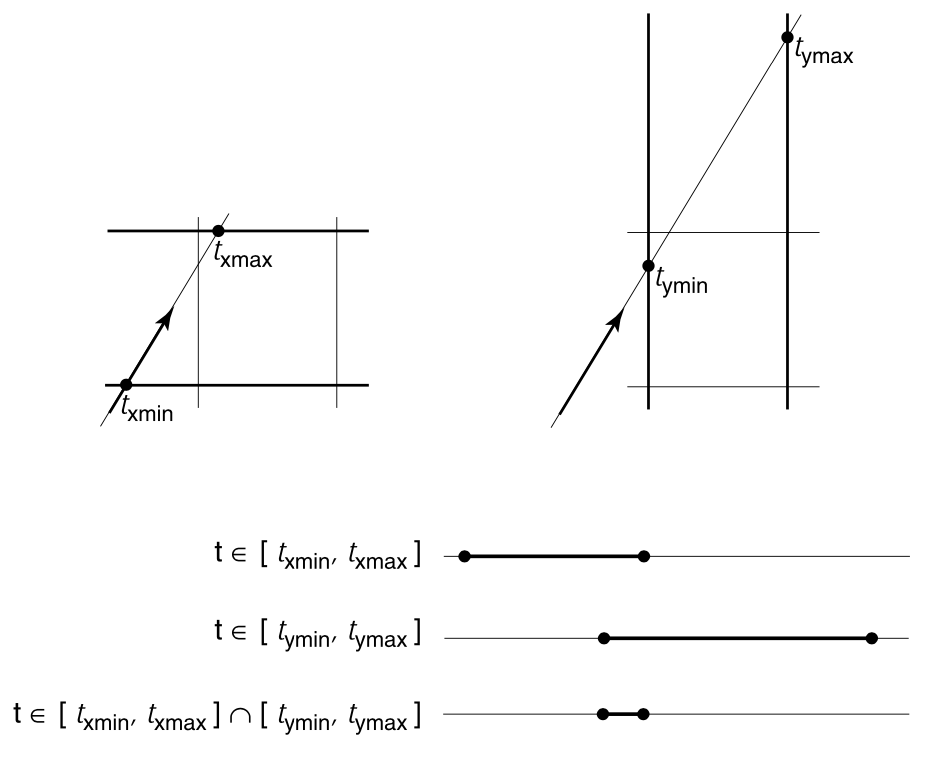
\includegraphics[width=0.7\textwidth]{figs/bounding box solve t}
	\caption{\label{bbt}2D Bounding Box Hit Criterion}
\end{figure}

\subsubsection{Handling Divide by Zero}
There is yet another concern that needs to be addressed in our formulation: divide by zero errors when $x_d = \pm 0$ or $y_d = \pm 0$. The detailed derivations can be found on pages 281 - 282 of the text book. We note the results here: 
\begin{equation}
	a = 1 / x_d, b = 1 / y_d
\end{equation}
\paragraph{If $(a \geq 0)$ then}
\begin{equation}
	t_{x\min} = a(x_{\min} - x_e); \quad t_{x\max} = a(x_{\max} - x_e)
\end{equation}
\vspace{-3em}
\paragraph{else}
\begin{equation}
	t_{x\min} = a(x_{\max} - x_e); \quad t_{x\max} = a(x_{\min} - x_e)
\end{equation}

\paragraph{If $(b \geq 0)$ then}
\begin{equation}
	t_{y\min} = b(y_{\min} - y_e); \quad t_{y\max} = b(y_{\max} - y_e)
\end{equation}
\vspace{-3em}
\paragraph{else}
\begin{equation}
	t_{y\min} = b(y_{\max} - y_e); \quad t_{y\max} = b(y_{\min} - y_e)
\end{equation}
Then, again, if $t_{x\min} > t_{y\max} \lor  t_{y\min} > t_{x\max} $ then the ray missed the bounding box. Otherwise, there is a hit. \footnote{This if statement condition could be derived from Figure \ref{bbt}: when the two intervals have no intersection, then we have a miss. }

\subsubsection{Handling 3D Bounding Boxes}
This is almost exactly the same as what we presented in the previous sub-subsection. We calculate a extra $c$ for the $z$ axis: $c = 1 / z_d$
\paragraph{If $(c \geq 0)$ then}
\begin{equation}
	t_{z\min} = c(z_{\min} - z_e); \quad t_{z\max} = c(z_{\max} - z_e)
\end{equation}
\vspace{-3em}
\paragraph{else}
\begin{equation}
	t_{z\min} = c(z_{\max} - z_e); \quad t_{z\max} = c(z_{\min} - z_e)
\end{equation}
However, this time the return conditions requires a bit more calculations
\begin{equation}
	lmin = \max\left\{ t_{\ast\min} \right\} \quad \text{is the largest of all min}
\end{equation}
and 
\begin{equation}
	smax = \min\left\{ t_{\ast\max} \right\} \quad \text{is the smallest of all max}
\end{equation}
Then, if $smax < lmin$, the ray missed the box; otherwise, there is a hit. 


%%%%%%%%%%%%%%%%%%%%%
% Meshes
%%%%%%%%%%%%%%%%%%%%%
\section{Meshes}
\subsection{Topology}
Topology is concerned with the connectivity of a mesh. We will assume that our meshes are 2-manifolds. A 2-manifold is a surface for which the neighbourhood around any point can be flattened onto the plane. 

\subsection{Watertight}
When a mesh have no holes, we say that it is water tight. On a similar note, meshes are \textit{\textbf{stricter}} then soups. When we have a triangle soup, we impose no limits on the connectivity between the neighbouring triangles - it could be disjoint everywhere.

\subsection{Geometry}
Geometrically, a mesh is a piecewise planar surface. It is 
\begin{itemize}
	\item planar almost everywhere, 
	\item except maybe at the edges where the triangles join. 
\end{itemize}
Very often, it is a piecewise planar approximation of a smooth surface. 







\end{document}
